\chapter{Approach}
\label{ch4_APPROACH}

This project aims at providing end to end system which takes inputs from
video activity recognizer and object detector to enhance the video activity recognition.

Figure \ref{fig:approach} explains the approach of this project.
\begin{figure}[H]
\begin{center}	
	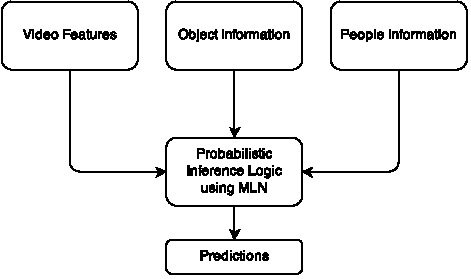
\includegraphics[scale=1.3]{approach} 
\caption{Approach of the Project}
\label{fig:approach}
\end{center}
\end{figure}

The video features are extracted as explained in section \ref{section_STIP}.
The code used in this phase is publicly made available at \cite{stipCode}.
Using one versus all (ovr) matlab interface of libsvm \cite{libsvm}, model is learnt to extract the 
confidence values from video feature classification.

The object features are evaluated using \cite{voc-release4}. 
Each object detection has a confidence value along with it.
This value is used to determine whether to consider detection
as a viable detection or spurious one. The thresholds for confidence
values are found experimentally. Details are given in chapter \ref{ch5_RESULTS}.

Main contribution of this project is in the formulation of
markov logic system. Alchemy \cite{alchemy2.0} software is
used to form markov logic network. The software allows convenient
representation of rules using first order logic and assigns weights to
such rules using the evidence provided. Following sections explain in detail
about the evidence creation, rules, etc.

\section{MLN Evidence}
The Hollywood2 data set \cite{hollywood2} (described in chapter \ref{ch5_RESULTS}) provides
true activity labels for training data. These labels are used to create predicates
like
\begin{equation}
	HasActivity( ``actioncliptrain00001", ``SitUp" )
\end{equation}

The learnt SVM model is used to classify training data set itself to get
confidence values of activities for all clips. These confidence values
are partitioned into bins to create predicates like
\begin{equation}
	\begin{split}
		~ & ActivityConf\_P1\_TO\_P15(``actioncliptrain00001",``SitUp") \\
		~ & ActivityConf\_NI\_TO\_N2(``actioncliptrain00002",``HandShake")
	\end{split}
\end{equation}

Here, P1\_TO\_P15 represents a bin with confidence value of +1 to +1.5.
Similarly other bins are formed and predicates are generated to form the evidence.
Each clip has 12 such predicates as there are 12 activity classes.

Object detector \cite{voc-release4} gives object detections in frames
along with the corresponding confidence values. Experimentally determined thresholds
are used to decide whether to consider object detection and predicates like following are formed
\begin{equation}
	\begin{split}
		~ & ObjPresent(``actioncliptrain00001",``person") \\
		~ & ObjPresent(``actioncliptrain00002",``car")
	\end{split}
\end{equation}

Finally, to generate evidence for people information, average number of ``person"
objects are calculated in each clip. These averages are partitioned into bins
and each clip is assigned one bin. Predicates like following are formed using this method
\begin{equation}
	\begin{split}
		~ & NumPersons\_1\_TO\_15(``actioncliptrain00001") \\
		~ & NumPersons\_0\_TO\_1(``actioncliptrain00002")
	\end{split}
\end{equation}





\section{MLN Rules}
For learning MLN model, rules corresponding to bins of confidence
from {\bf video classifier} are written.
For example,
\begin{equation}
	\begin{split}
		ActivityConf\_N1\_TO\_N05(clip,activity) \implies & HasActivity(clip,activity) \\
		ActivityConf\_P1\_TO\_P15(clip,activity) \implies & HasActivity(clip,activity)
	\end{split}
\end{equation}

Here, the $1^{st}$ rule captures relation between low confidence ($-1$ to $-0.5$) of presence
of activity and actual evidence. And $2^{nd}$ rule captures relation between
higher confidence ($+1$ to $+1.5$) of presence of activity and actual evidence.
Thus intuitively, $1^{st}$ rule will get lower weight as compared to $2^{nd}$ rule.

~ \\
For adding {\bf object information}, both positive and negative rules are written.
Positive rules are intuitive rules which enhance the probability of likely
inference. Negative rules are counter intuitive rules which suppress the
probability of unlikely rules. In both the types, the confidence of classification
improves. Below is example of few positive rules
\begin{equation}
	\begin{split}
		ObjPresent(c,``chair") \implies & HasActivity(c,``Eat") \\
		ObjPresent(c,``car") \implies & HasActivity(c,``DriveCar")
	\end{split}
\end{equation}
and few negative rules
\begin{equation}
	\begin{split}
		ObjPresent(c,``bus") \implies & HasActivity(c,``StandUp") \\
		ObjPresent(c,``car") \implies & HasActivity(c,``HandShake")
	\end{split}
\end{equation}

~ \\
For learning relationship between {\bf people information} and activities,
rules consisting of bins of number of people and activities are written.
For example,
\begin{equation}
	\begin{split}
		NumPersons\_0\_TO\_1(clip)\implies & HasActivity(clip,+a) \\
		NumPersons\_1\_TO\_15(clip)\implies & HasActivity(clip,+a)
	\end{split}
\end{equation}

where, $1^{st}$ rule has a bin that corresponds to average number of people 
per frame between 0 to 1.
``+a" means rule will be expanded to all possible activities. Thus for each bin,
rules corresponding to all 12 activities will be used in MLN learning.




\section{MLN Inference}
For inference, the learnt SVM model is used to classify testing
data set clips. This step provides with the confidence values of activities for
each clip. These confidence values are partitioned into bins in same manner
as done for generating evidence.
The object and people information is added in similar fashion as that of
evidence generation process. 

Inference is made on predicate ``HasActivity". Thus only difference
between evidence and inference is absence of ``HasActivity" predicates.

Sample inference instance looks like
\begin{equation}
	\begin{split}
		~ & ActivityConf\_P1\_TO\_P15(``actioncliptest00001",``Kiss") \\
		~ & ActivityConf\_N2\_TO\_N15(``actioncliptest00002",``Eat") \\
		~ & ObjPresent(``actioncliptest00001",``person") \\
		~ & ObjPresent(``actioncliptest00002",``person") \\
		~ & NumPersons\_2\_TO\_I(``actioncliptest00001") \\
		~ & NumPersons\_1\_TO\_15(``actioncliptest00002") \\
		~ & \vdots
	\end{split}
\end{equation}

~ \\
{\bf AAP Calculations - }Using the probabilities given by MLN inference, inferred activity for each
clip is determined corresponding to maximum probability. The data set provides with true activity labels for test clips. 
These true activities and MLN inferred activities are used to calculate average average precision
of MLN system. Next chapter shows the results.

